\documentclass{beamer}

% theme definition
\usetheme{KU}

\usepackage{natbib}
\usepackage{alltt}
\usepackage{trust}
\usepackage{fixltx2e}
\usepackage{amsmath}
%\usepackage{trust-spi}
\usepackage{tikz}
\usetikzlibrary{arrows,shadows, matrix}
\usepackage[underline=false]{pgf-umlsd}
\usepackage{graphicx}

\usepackage{listings}
\lstset{language=Haskell, emph={main, Request, CAResponse, CACertificate, EvidencePackage, Response, Att,TPM_KEY ,TPM_KEY_USAGE
    , TPM_KEY_FLAGS
    , TPM_AUTH_DATA_USAGE
    , TPM_KEY_PARMS
    , ByteString
    , TPM_STORE_PUBKEY, OIAP, OSAP, TPM_NONCE, TPM_DIGEST, TPM_QUOTE_INFO, TPM_COMPOSITE_HASH, Binary, Get, TPM_STRUCT_VER, TPM, TPM_KEY_HANDLE, TPM_KEY, Session}, emphstyle=\textbf, deletekeywords={putStrLn, Handle}, showstringspaces=false}
\lstset{%
  literate={->}{{ ${\rightarrow}$ }}3 {<-}{{ $\leftarrow$ }}3 
}

\setbeamertemplate{blocks}[rounded][shadow=true]

\setbeamercolor{title}{fg=kublue}
\setbeamercolor{subtitle}{fg=kugray} 
\setbeamercolor{institute}{fg=kugray}
\setbeamercolor{frametitle}{fg=kublue}
\setbeamercolor{frametitle}{bg=white}
\setbeamercolor{framesubtitle}{fg=kugray}
\setbeamercolor{framesubtitle}{bg=white}
\setbeamercolor{item}{fg=black}
\setbeamercolor{subitem}{fg=kugray}
\setbeamercolor{itemize/enumerate subbody}{fg=kugray}
\setbeamercolor{block title}{bg=kublue}
\setbeamercolor{block title}{fg=white}
\setbeamercolor{block body}{bg=sand}
\setbeamercolor{block body}{fg=black}

\setbeamertemplate{footline}[frame number]

\usefonttheme{serif}

\newenvironment{fnverbatim}{\begin{alltt}\scriptsize}{\normalsize\end{alltt}}
\newcommand{\mean}[1]{\langle#1\rangle}
\newcommand{\rtime}{\ensuremath{\mathbb{R}^{0\leq}}}


%constants
\def \app {App}
\def \att {Att}
\def \ca {CA}
\def \mea {Meas}
\def \tp {TPM}
\def \pmask {PCR\textsubscript{m}}
\def \pcomp {PCR\textsubscript{c}}
\def \evd {d}
\def \eve {e}
\def \cacert {\sign {\public{AIK}}{CA}}
\def \exdata {\hash{(\eve, \nonce{\app}, \cacert ) }}
\def \aikh {AIK_h}

\def \req {R}
\def \resp {P}
\def \k {K}

\bibliographystyle{apalike}

\logo{}

\title{ArmoredSoftware}
\subtitle{User-Space Remote Attestation}

\author{Dr. Perry Alexander\inst{1} \and Dr. Andrew Gill\inst{1} \and Dr. Prasad
  Kulkarni\inst{1} \and
  Adam Petz\inst{1} \and Paul Kline\inst{1} \and Justin Dawson\inst{1}
  \and Jason~Gevargizian\inst{1} 
  \and Leon Searl\inst{1} \and Edward Komp\inst{1} \and
  Edward~Bishop\inst{2} \and Ciro Pinto-Coelho\inst{2}} 

\date{{\color{kugray}May 1, 2015}}

% turns off navigation symbols
\setbeamertemplate{navigation symbols}{}

\institute{
  \inst{1}
    Information and Telecommunication Technology Center \\
    Electrical Engineering and Computer Science \\
    The University of Kansas \\
    \medskip
  \inst{2} Southern Cross Engineering}

\begin{document}

\begin{frame}
  \titlepage
\end{frame}

%\logo{\pgfuseimage{jhwk4C_RF}}

% \begin{frame}
%   \frametitle{Outline}
%   \tableofcontents
% \end{frame}

\section{Introduction and Project Goals}

\begin{frame}
  \frametitle{Clouds and Trust}
  \begin{itemize}
  \item The promises of ``the cloud'' are substantial
    \begin{itemize}
    \item reduced hardware and software costs
    \item reduced resource consumption
    \item improved availability and reliability
    \end{itemize}
  \item The promises of ``the cloud'' complicate assurance
    \begin{itemize}
    \item not under the desk
    \item ambiguous and changing runtime environment
    \item unknown and unknowable actors in the same environment
    \end{itemize}
  \item Is trust possible in ``the cloud'' environment?
    \begin{itemize}
    \item unambiguous identification
    \item confirmation of uninhibited execution
    \item direct or trusted indirect observation of good behavior  
    \end{itemize}
  \end{itemize}
\end{frame}

\begin{frame}
  \frametitle{Program Goals}
  \framesubtitle{Virtual Blinking Lights}
  \begin{block}{Trust in the Cloud}
    Provide new capabilities that establish and maintain trustworthy
    cloud-based application deployment
  \end{block}
  \begin{itemize}
  \item Establish trust among cloud components
    \begin{itemize}
    \item trust among cohorts of processes
    \item trust among processes and environment
    \end{itemize}
  \item Promote informed decision making
    \begin{itemize}
    \item data confidentiality can be confirmed
    \item execution and data integrity can be confirmed
    \end{itemize}
  \item Autonomous run-time response and reconfiguration
    \begin{itemize}
    \item responds to attack, failure, reconfiguration, and repair 
    \item response varies based on measurement
    \end{itemize}
  \end{itemize}
\end{frame}

\begin{frame}
  \frametitle{Delivery Platform}
  \framesubtitle{Open source, standards compliant}

  \begin{itemize}
  \item Lightweight integration with existing cloud infrastructure
    \begin{itemize}
    \item OpenStack cloud infrastructure
    \item Xen+XSM VM infrastructure
    \item Fedora, HotSpot JVM, GHC
    \end{itemize}
  \item Trusted Computing Group standards compliant
    \begin{itemize}
    \item Trusted Platform Module 1.2
    \item TCG vTPM (in principle)
    \item Trusted OS infrastructure
    \end{itemize}
  \item Standard communication mechanisms
    \begin{itemize}
    \item JSON structures for all exchanged data
    \item \textsl{vchan} for on-platform communication
    \item TCP/IP for off-platform communication
    \end{itemize}
  \end{itemize}
\end{frame}

\begin{frame}
  \frametitle{New Technologies}
  \begin{itemize}
  \item Trustworthy protocol execution
    \begin{itemize}
    \item executable protocol representation
    \item protocol execution generates evidence of trustworthiness
    \item highly focused protocols
    \item strand space formal semantics
    \end{itemize}
  \item Application specific measurement
    \begin{itemize}
    \item managed and traditional execution environments
    \item compile-time assistance for measurer synthesis
    \item specialized measurement bundled with applications
    \end{itemize}
  \item Attestation driven cloud application and data management
    \begin{itemize}
    \item health monitoring
    \item problem mitigation
    \item application migration
    \item access control
    \end{itemize}
  \end{itemize}
\end{frame}

% \begin{frame}
%   \frametitle{Research \& Development Plan}
%   \begin{itemize}
%   \item Development and integrate measurement capabilities
%     \begin{itemize}
%     \item hosted languages (Java)
%     \item traditional compiled languages (C, C++)
%     \item integrate with environment measurers (Xen,OpenStack,OS)
%     \end{itemize}
%   \item Develop attestation capabilities
%     \begin{itemize}
%     \item flexible, user configurable protocol representation
%     \item measured protocol execution
%     \item protocol execution appraisal
%     \end{itemize}
%   \item Develop infrastructure trust argument
%     \begin{itemize}
%     \item develop lightweight vTPM infrastructure supporting mobility
%     \item launch from known roots of trust
%     \item maintain trust evidence at run time
%     \item maintain trust over migration
%     \end{itemize}
%   \end{itemize}
% \end{frame}

% \begin{frame}
%   \frametitle{Research \& Development Plan}
%   \begin{itemize}
%   \item Automated synthesis and verification
%     \begin{itemize}
%     \item measurer synthesis at application compile time
%     \item automated evidence appraisal from protocols
%     \item formal trust argument
%     \end{itemize}
%   \item Demonstrations
%     \begin{itemize}
%     \item initial simple infrastructure demonstrations
%     \item cloud-based ``big data'' environment demonstration
%     \item federated trust demonstration
%     \item \emph{demonstrations as discovered/directed}
%     \end{itemize}
%   \item Scale up and roll out
%     \begin{itemize}
%     \item integration with Xen, OpenStack, Linux
%     \item installation management and packaging
%     \item effective web presence
%     \end{itemize}
%   \end{itemize}
% \end{frame}

\begin{frame}
  \frametitle{Trusted Platform Module}
  \begin{itemize}
  \item Provides and Protects Roots of Trust
    \begin{itemize}
    \item Storage Root Key (SRK) - root of trust for storage
    \item Endorsement Key (EK) - root of trust for reporting
    \end{itemize}
  \item Quote generation
    \begin{itemize}
    \item high integrity quotes - (\sign{RS}{AIK}, SML, \sign{n,PCRComp}{AIK})
    \item high integrity evidence - (\tuple{E,n}, \sign{\hash{\tuple{E,n}},PCR}{AIK}
    \end{itemize}
  \item Sealing data to state
    \begin{itemize}
    \item \encrypt{D,PCR}{K} will not decrypt unless PCR = current PCR
    \item data is safe even in the presence of malicious machine
    \end{itemize}
  \item Binding data to TPMs and machines
    \begin{itemize}
    \item (\encrypt{\private{K}}{SRK},K) - \encrypt{D}{K} cannot be decrypted unless \private{SRK} is installed
    \item (\encrypt{\private{J}}{K},J) - \encrypt{D}{J} cannot be decrypted
      unless \private{K} and \private{SRK} are installed
    \end{itemize}
  \end{itemize}
\end{frame}

\section{System Architecture}

\begin{frame}
  \frametitle{Semantic Remote Attestation}

  \begin{columns}[c]
    \column{0.55\textwidth}
    \begin{itemize}
    \item Appraiser requests a quote
      \begin{itemize}
      \item specifies needed information
      \item provides a nonce
      \end{itemize}
    \item Target gathers evidence
      \begin{itemize}
      \item measures application
      \item gathers evidence of trust
      \end{itemize}
    \item Target generates quote
      \begin{itemize}
      \item measurements and evidence
      \item original nonce
      \item cryptographic signature
      \end{itemize}
    \item Appraiser assesses quote
      \begin{itemize}
      \item good application behavior
      \item infrastructure trustworthiness
      \end{itemize}
    \end{itemize}
    \column{0.45\textwidth}
    \begin{center}
      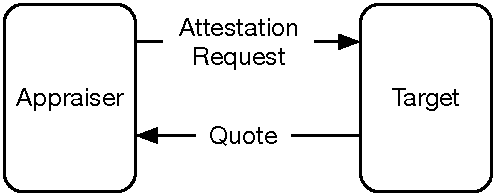
\includegraphics[width=.95\textwidth]{figures/remote-att.pdf}
    \end{center}
  \end{columns}
\end{frame}

\begin{frame}
  \frametitle{Armored Application Architecture}
  \begin{columns}[c]
    \column{.60\textwidth}
    \begin{itemize}
    \item Focus is user-space applications
    \item Assesses the cloud infrastructure and environment
    \item Attests to the state of its application
    \item High-assurance, lightweight infrastructure
    \item Influenced by the \emph{Trusted Research Platform} and
      \emph{Principles of Remote Attestation}
    \end{itemize}
    \column{.40\textwidth}
    \begin{center}
    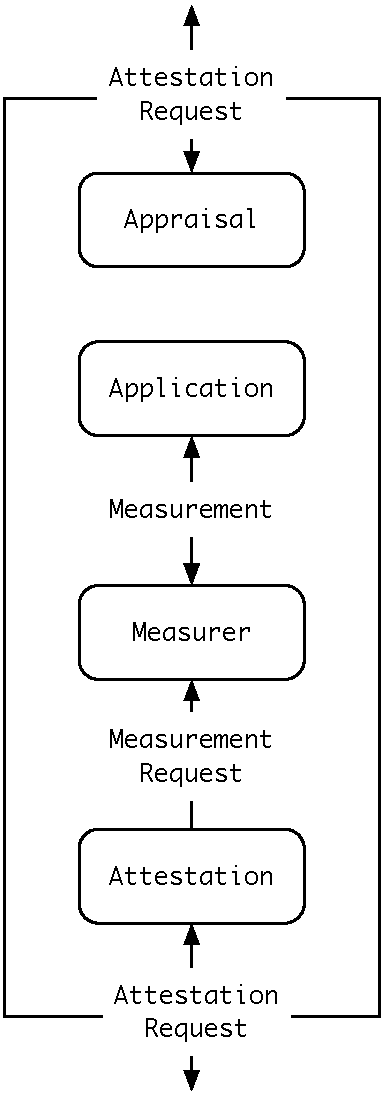
\includegraphics[width=0.55\textwidth]{figures/architecture.pdf}
    \end{center}
  \end{columns}
\end{frame}

\begin{frame}
  \frametitle{Measurement and Attestation}
  \begin{center}
  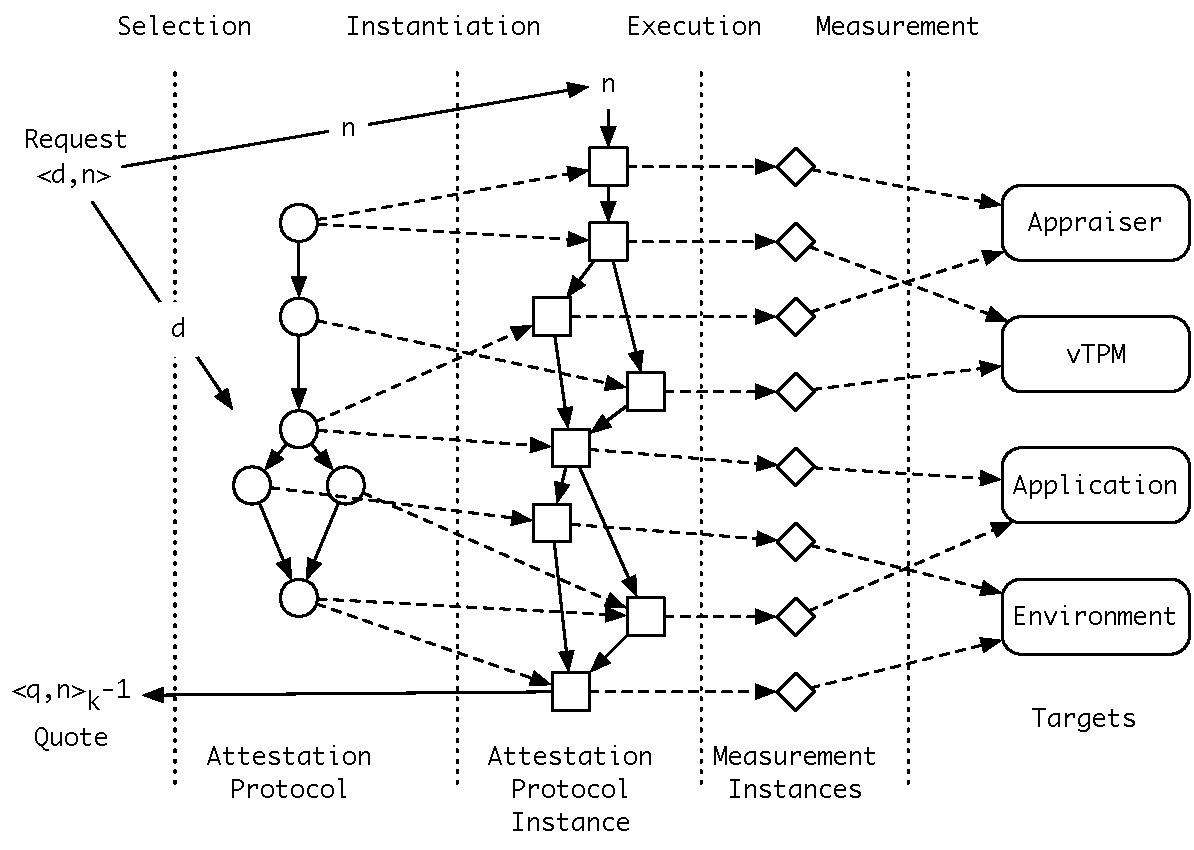
\includegraphics[width=0.9\textwidth]{figures/ap-1.pdf}
  \end{center}
\end{frame}

\begin{frame}
  \frametitle{System-Level Architecture}
  \begin{center}
  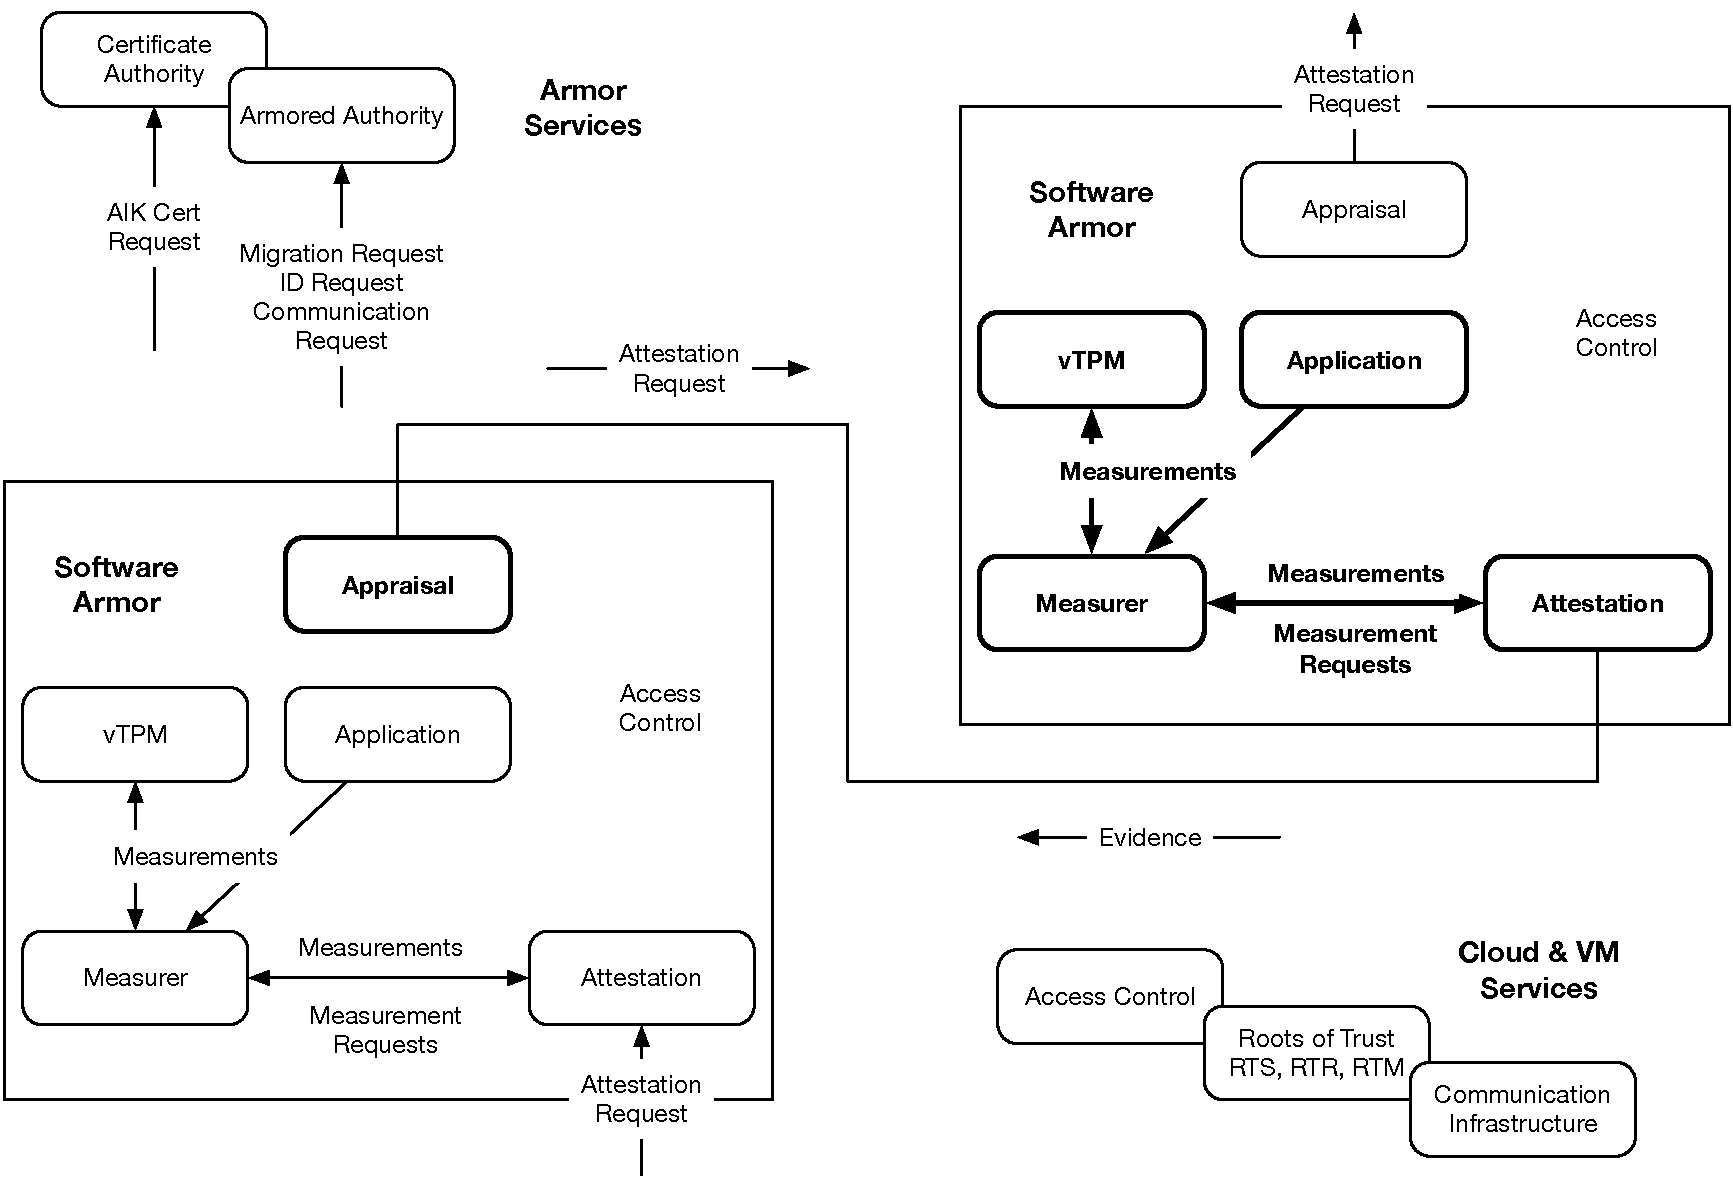
\includegraphics[width=0.9\textwidth]{figures/system.pdf}
  \end{center}
\end{frame}

\section{Prototype demonstration and discussion}

% \begin{frame}
%   \frametitle{What We Are Demonstrating}
  
%   \begin{itemize}
%   \item Execution of a CA-based Attestation Protocol
%     \begin{itemize}
%     \item Attestation request
%     \item Protocol execution
%     \item Evidence appraisal
%     \end{itemize}
%   \item Major architectural subsystems
%     \begin{itemize}
%     \item Appraiser
%     \item Attestation Manager
%     \item Measurer
%     \item Instrumented JVM
%     \item vTPM and Certificate Authority
%     \end{itemize}
%   \item Anomaly Detection
%     \begin{itemize}
%     \item Bad signatures and PCRs
%     \item Bad CA certificates
%     \item Bad quotes and AIKs
%     \item Bad measurements
%     \end{itemize}
%   \end{itemize}
% \end{frame}

% \begin{frame}[fragile]
%   \frametitle{Abstract CA-Based Attestation Protocol}

%   \begin{center}

%     \begin{tikzpicture}[
%     implies/.style={double,double equal sign distance,-implies},
%     dot/.style={shape=circle,fill=black,minimum size=4pt,
%       inner sep=0pt,outer sep=4pt}]

%     \matrix[matrix of nodes] {
%       |[dot,label=above:$\app$] (A1)| {}
%       &[2.0cm] |[dot,label=above:$\att$] (B1)| {}
%       &[2.0cm] |[] (M1)| {} 
%       &[2.0cm] |[] (T1)| {}\\[0.05cm]
%       |[] (A2)| {}
%       &|[dot] (B2)| {}
%       &|[dot,label=above:$\mea$] (M2)| {} 
%       &|[] (T2)| {}\\[0.05cm]
%       |[] (A3)| {}
%       &|[] (B3)| {}
%       &|[dot] (M3)| {} 
%       &|[dot,label=above:$Tar$] (T3)| {}\\[0.6cm]
%       |[] (A4)| {}
%       &|[] (B4)| {}
%       &|[dot] (M4)| {} 
%       &|[dot] (T4)| {}\\[0.6cm]
%       |[] (A5)| {}
%       &|[dot] (B5)| {}
%       &|[dot] (M5)| {} 
%       &|[] (T5)| {}\\[0.6cm]
%       |[dot] (A6)| {}
%       &[2.0cm] |[dot] (B6)| {}
%       &[2.0cm] |[] (M6)| {} 
%       &[2.0cm] |[] (T6)| {}\\
%     };
%     \draw (A1) edge[->] node[above] {request} (B1);
%     \draw (B2) edge[->] node[above] {request} (M2)
%            edge[implies,implies-] (B1);
%     \draw (M3) edge[->] node[above] {request} (T3)
%            edge[implies,implies-] (M2);
%     \draw (T4) edge[->] node[above] {measurement} (M4)
%            edge[implies,implies-] (T3);
%     \draw (M5) edge[->] node[above] {evidence} (B5)
%            edge[implies,implies-] (M4);
%     \draw (B6) edge[->] node[above] {quote} (A6)
%            edge[implies,implies-] (B5);
%     \end{tikzpicture}

%     \end{center}

% \end{frame}

% \begin{frame}
%   \frametitle{Abstract CA-Based Attestation Protocol}
  
%   \begin{footnotesize}
%   \begin{sequencediagram}
%     \newthread[white]{appr}{Appraiser}
%     \newinst[0.7]{attest}{Attestation}
%     \newinst[0.7]{ca}{CA}
%     \newinst[0.7]{meas}{Measurer}
%     \newinst[0.7]{app}{Application}
    
%     \begin{call}{appr}{Att Request}{attest}{Evidence}
%       \begin{call}{attest}{Cert Request}{ca}{AIK Cert}
%       \end{call}
%       \begin{call}{attest}{Measurement Request}{meas}{Value}
%         \begin{call}{meas}{Measurement}{app}{Value}
%         \end{call}
%       \end{call}
%       \begin{callself}{attest}{Quote Assembly}{}
%       \end{callself}
%     \end{call}
%     \begin{callself}{appr}{Appraisal}{Execute Decision}
%     \end{callself}
%   \end{sequencediagram}
%   \end{footnotesize}

% \end{frame}

% \begin{frame}
%   \frametitle{Message List Representation}
%   \begin{small}
%   \begin{align*}
%   & \sndmsg {\app}{\att} {\evd, \nonce{\app}, \pmask} {\channel {\app \att}}  & \\
%   & \sndmsg{\att}{\tp} {make\_and\_load\_identity} {\channel {\att \tp}} & \\
%   & \sndmsg{\tp}{\att} {\public{AIK}, \aikh} {\channel {\tp \att}} & \\
%   & \sndmsg{\att}{\ca} {\att, \public{AIK}} {\channel {\att \ca}} & \\
%   & \sndmsg{\ca}{\att} {\encrypt{K, \hash{AIK}}{EK}, \encrypt{\cacert}{K}} {\channel {\ca \att}}& \\
%   & \sndmsg{\att}{\tp} {activate\_identity({\aikh, \hash{AIK})}} {\channel {\att \tp}} & \\
%   & \sndmsg{\tp}{\att} {K} {\channel {\tp \att}} & \\
%   & \sndmsg{\att}{\mea} {\evd} {\channel {\att \mea}} & \\
%   & \sndmsg{\mea}{\att} {\eve} {\channel {\mea \att}} & \\
%   & \sndmsg{\att}{\tp} {quote(\;{AIK\textsubscript{h}, \pmask, \exdata}\;)} {\channel {\att \tp}} & \\
%   & \sndmsg{\tp}{\att} {\pcomp, \sign{\hash{\pcomp}, \exdata}{AIK}} {\channel {\tp \att}} & \\
%   & \sndmsg{\att}{\app} {\eve, \nonce{\app}, \pcomp, \cacert} {\channel {\att \app}} & \\
%   & \sndmsg{\att}{\app} {\sign{\hash{\pcomp}, \exdata}{AIK}} {\channel {\att \app}} & 
% \end{align*}
% \end{small}
% \end{frame}



\begin{frame}[fragile]
  \frametitle{Privacy CA Attestation}

  \begin{tiny}
  \begin{tikzpicture}[
    implies/.style={double,double equal sign distance,-implies},
    dot/.style={shape=circle,fill=black,minimum size=4pt,
      inner sep=0pt,outer sep=4pt}]

    \matrix[matrix of nodes] {
      |[dot,label=above:$\app$] (A1)| {}
      &[4.0cm] |[dot,label=above:$\att$] (B1)| {}
      &[1.95cm] |[] (M1)| {} 
      &[1.95cm] |[] (T1)| {}
      &[0.5cm] |[] (C1)| {}\\[0.05cm]
      & |[dot] (B2)| {}
      &
      & |[dot,label=above:$\tp$] (T2)| {}\\[0.5cm]
      &
      |[dot] (B3)| {}
      &
      & |[dot] (T3)| {}\\  [0.05cm]
      &
      |[dot] (B4)| {}
      &
      &
      & |[dot,label=above:$\ca$] (C4)| {} \\ [0.5cm]
      &
      |[dot] (B5)| {}
      &
      &
      & |[dot] (C5)| {} \\ [0.5cm]
      &
      |[dot] (B6)| {}
      &
      & |[dot] (T6)| {} \\ [0.5cm]
      &
      |[dot] (B7)| {}
      &
      & |[dot] (T7)| {} \\ [0.05cm]
      &
      |[dot] (B8)| {}
      & |[dot,label=above:$\mea$] (M8)| {} \\ [0.5cm]
      &
      |[dot] (B9)| {}
      & |[dot] (M9)| {} \\ [0.5cm]
      &
      |[dot] (B10)| {}
      &
      & |[dot] (T10)| {} \\ [0.5cm]
      &
      |[dot] (B11)| {}
      &
      & |[dot] (T11)| {} \\ [0.5cm]
      |[dot] (A12)| {}
      & |[dot] (B12)| {} \\ [0.5cm]
      |[dot] (A13)| {}
      & |[dot] (B13)| {} \\ [0.5cm]
};
\draw (A1) edge[->] node[above] {$\evd, \nonce{\app}, \pmask$} (B1);
\draw (B2) edge[->] node[above] {$make\_and\_load\_identity$} (T2)
           edge[implies,implies-] (B1);
\draw (T3) edge[->] node[above] {$\aikh$} (B3)
           edge[implies,implies-] (T2);
\draw (B4) edge[->] node[above] {$\public{AIK}$} (C4)
           edge[implies,implies-] (B3);
\draw (C5) edge[->] node[above] {$\encrypt{K, \hash{\public{AIK}}}{EK}, \crypt{\cacert}{K}$} (B5)
           edge[implies,implies-] (C4);
\draw (B6) edge[->] node[above] {$activate\_identity(\aikh, \encrypt{K, \hash{\public{AIK}}}{EK})$} (T6)
           edge[implies,implies-] (B5);
\draw (T7) edge[->] node[above] {$K$} (B7)
           edge[implies,implies-] (T6);
\draw (B8) edge[->] node[above] {$\evd$} (M8)
           edge[implies,implies-] (B7);
\draw (M9) edge[->] node[above] {$\eve$} (B9)
           edge[implies,implies-] (M8);
\draw (B10) edge[->] node[above] {$quote(\;\aikh, \pmask, \exdata \;)$} (T10)
% quote(\;{AIK\textsubscript{h}, \pmask, \exdata}\;)
           edge[implies,implies-] (B9);
\draw (T11) edge[->] node[above] {$\pcomp, \sign{\hash{\pcomp}, \exdata}{AIK}$} (B11)
% \pcomp, sig(\hash{\pcomp}, ed) AIK
           edge[implies,implies-] (T10);
\draw (B12) edge[->] node[above] {$\eve, \nonce{\app}, \pcomp, \cacert$} (A12)
% \eve, \nonce{\app}, \pcomp, \cacert
           edge[implies,implies-] (B11);
\draw (B13) edge[->] node[above] {$\sign{\hash{\pcomp}, \exdata}{AIK}$} (A13) 
% sig(hash(\pcomp), ed) AIK
           edge[implies,implies-] (B12);
\end{tikzpicture}
\end{tiny}
\end{frame}

% \begin{frame}[fragile]
%   \frametitle{Attestation Request}
%   \begin{center}
%     \begin{tikzpicture}[
%       implies/.style={double,double equal sign distance,-implies},
%       dot/.style={shape=circle,fill=black,minimum size=4pt,
%         inner sep=0pt,outer sep=4pt}]
%       \matrix[matrix of nodes] {
%         |[dot,label=above:$\app$] (A1)| {}
%         &[7.5cm] |[dot,label=above:$\att$] (B1)| {} \\ [1.0cm]
%       };
%       \draw (A1) edge[->] node[above] {$\evd, \nonce{\app}, \pmask$} (B1);
%     \end{tikzpicture}
%   \end{center}

%     \begin{itemize}
%     \item Initiate with an attestation request
%       \begin{itemize}
%       \item $d$ abstractly defines desired evidence
%       \item $\nonce{\app}$ is the appraiser's nonce
%       \item $\pmask$ selects PCRs
%       \end{itemize}
%     \item Attestation agent selects and executes protocol based on request
%     \end{itemize}
% \end{frame}

% \begin{frame}[fragile]
%   \frametitle{Generating and Certifying an AIK}

%   \begin{columns}[c]
%     \column{.45\textwidth}
%     \begin{small}
%     \begin{itemize}
%     \item Request a new $AIK$ from TPM (optional)
%     \item Receive $AIK$ handle
%     \item Request $\public{AIK}$ signed by CA ($AIK$ cert)
%     \item Receive $AIK$ cert encrypted with session key $K$
%     \item Receive $K$ encrypted with public $EK$
%     \end{itemize}
%     \end{small}
%     \column{.55\textwidth}
%     \begin{small}
%     \begin{tikzpicture}[
%       implies/.style={double,double equal sign distance,-implies},
%       dot/.style={shape=circle,fill=black,minimum size=4pt,
%         inner sep=0pt,outer sep=4pt}]
%       \matrix[matrix of nodes] {
%         |[dot,label=above:$\att$] (B2)| {}
%         &[3.5cm] |[dot,label=above:$\tp$] (T2)| {}\\[1.0cm]
%         &[0.5cm] |[] (C2)| {}\\[0.5cm]
%         |[dot] (B3)| {}
%         & |[dot] (T3)| {}\\  [0.5cm]
%         |[dot] (B4)| {}
%         &
%         & |[dot,label=above:$\ca$] (C4)| {} \\ [1.0cm]
%         |[dot] (B5)| {}
%         &
%         & |[dot] (C5)| {} \\ [0.5cm]
%       };
% \draw (B2) edge[->] node[above] {$make\_and\_load\_identity$} (T2);
% \draw (T3) edge[->] node[above] {$\aikh$} (B3)
%            edge[implies,implies-] (T2);
% \draw (B4) edge[->] node[above] {$\public{AIK}$} (C4)
%            edge[implies,implies-] (B3);
% \draw (C5) edge[->] node[above] {$\encrypt{K, \hash{\public{AIK}}}{EK}, \crypt{\cacert}{K}$} (B5)
%            edge[implies,implies-] (C4);
%     \end{tikzpicture}
%     \end{small}
%   \end{columns}
% \end{frame}

% \begin{frame}[fragile]
%   \frametitle{Activating the AIK}

%   \begin{center}
%     \begin{tikzpicture}[
%       implies/.style={double,double equal sign distance,-implies},
%       dot/.style={shape=circle,fill=black,minimum size=4pt,
%         inner sep=0pt,outer sep=4pt}]
%       \matrix[matrix of nodes] {
%         |[dot,label=above:$\att$] (B6)| {}
%         &[7.5cm] |[dot,label=above:$\tp$] (T6)| {} \\ [1.0cm]
%         |[dot] (B7)| {}
%         &|[dot] (T7)| {} \\
%       };
% \draw (B6) edge[->] node[above] {$activate\_identity(\aikh, \encrypt{K, \hash{\public{AIK}}}{EK})$} (T6);
% \draw (T7) edge[->] node[above] {$K$} (B7)
%            edge[implies,implies-] (T6);
%     \end{tikzpicture}
%   \end{center}

%     \begin{itemize}
%     \item Request TPM decryption of the $AIK$ cert
%     \item Receive $K$ used to decrypt signed public $AIK$
%     \item Only TPM can gain access to $K$
%     \item Only TPM can obtain signed, public $AIK$
%     \item Oddly, No manipulation of the $AIK$ in this ``activation''
%       process
%     \end{itemize}

% \end{frame}

% \begin{frame}[fragile]
%   \frametitle{Measurement}

%   \begin{center}
%     \begin{tikzpicture}[
%       implies/.style={double,double equal sign distance,-implies},
%       dot/.style={shape=circle,fill=black,minimum size=4pt,
%         inner sep=0pt,outer sep=4pt}]
%       \matrix[matrix of nodes] {
%         |[dot,label=above:$\att$] (B8)| {}
%         &[7.5cm] |[dot,label=above:$\mea$] (M8)| {} \\ [1.0cm]
%         |[dot] (B9)| {}
%         &|[dot] (M9)| {} \\
%       };
%       \draw (B8) edge[->] node[above] {$\evd$} (M8);
%       \draw (M9) edge[->] node[above] {$\eve$} (B9)
%       edge[implies,implies-] (M8);
%     \end{tikzpicture}
%   \end{center}

%     \begin{itemize}
%     \item Request information from measurer
%     \item Receive evidence $e$ from measurer
%     \item $d$ is abstract allowing protocol reuse
%     \item Most protocols make many requests of the measurer
%     \end{itemize}

% \end{frame}

% \begin{frame}[fragile]
%   \frametitle{Generating a Quote}

%   \begin{center}
%     \begin{tikzpicture}[
%       implies/.style={double,double equal sign distance,-implies},
%       dot/.style={shape=circle,fill=black,minimum size=4pt,
%         inner sep=0pt,outer sep=4pt}]
%       \matrix[matrix of nodes] {
%         |[dot,label=above:$\att$] (B10)| {}
%         &[7.5cm] |[dot,label=above:$\tp$] (T10)| {} \\ [1.0cm]
%         |[dot] (B11)| {}
%         &|[dot] (T11)| {} \\
%       };
% \draw (B10) edge[->] node[above] {$quote(\;\aikh, \pmask, \exdata \;)$} (T10);
% % quote(\;{AIK\textsubscript{h}, \pmask, \exdata}\;)
% \draw (T11) edge[->] node[above] {$\pcomp, \sign{\hash{\pcomp}, \exdata}{AIK}$} (B11)
% % \pcomp, sig(\hash{\pcomp}, ed) AIK
%            edge[implies,implies-] (T10);
%     \end{tikzpicture}
%   \end{center}

%     \begin{itemize}
%     \item Request a quote from the TPM
%       \begin{itemize}
%       \item $AIK$ identifies the signing $AIK$
%       \item $PCR_m$ identifies desired PCRs
%       \item $\exdata$ guarantees integrity of returned evidence
%       \end{itemize}
%     \item Receive quote from TPM
%       \begin{itemize}
%       \item $\pcomp$ is PCR composite built from requested PCRs
%       \item $\sign{\hash{\pcomp}, \exdata}{AIK}$ is the signed quote
%       \end{itemize}
%     \end{itemize}

% \end{frame}

% \begin{frame}[fragile]
%   \frametitle{Appraisal}

%   \begin{center}
%     \begin{tikzpicture}[
%       implies/.style={double,double equal sign distance,-implies},
%       dot/.style={shape=circle,fill=black,minimum size=4pt,
%         inner sep=0pt,outer sep=4pt}]
%       \matrix[matrix of nodes] {
%         |[dot,label=above:$\app$] (A12)| {}
%         &[7.5cm] |[dot,label=above:$\att$] (B12)| {} \\ [1.0cm]
%         |[dot] (A13)| {}
%         &|[dot] (B13)| {} \\
%       };
%       \draw (B12) edge[->] node[above] {$\eve, \nonce{\app}, \pcomp, \cacert$} (A12);
%       % \eve, \nonce{\app}, \pcomp, \cacert
% \draw (B13) edge[->] node[above] {$\sign{\hash{\pcomp}, \exdata}{AIK}$} (A13) 
% % sig(hash(\pcomp), ed) AIK
%            edge[implies,implies-] (B12);

%     \end{tikzpicture}
%   \end{center}

%     \begin{itemize}
%     \item Receive evidence from the attestation manager
%       \begin{itemize}
%       \item evidence
%       \item original nonce
%       \item PCR composite 
%       \item signed $\public{AIK}$
%       \end{itemize}
%     \item Receive TPM quote from the attestation manager
%       \begin{itemize}
%       \item hash of all evidence
%       \item PCR composite
%       \item signed by $\private{AIK}$
%       \end{itemize}
%     \item Evaluate evidence and quote
%     \end{itemize}

% \end{frame}

% \begin{frame}
%   \frametitle{Evidence Appraisal}

%   \begin{center}
%     {\color{kublue}Demonstration detects failure of all aspects of attestation}
%   \end{center}

%   \[\eve, \nonce{\app}, \pcomp, \cacert\]

%   \begin{itemize}
%   \item $\eve$ -- evidence gathered from running application
%   \item $\nonce{\app}$ -- prevents replay
%   \item $\pcomp$ -- evidence in the form or PCR data from the vTPM
%   \item $\cacert$ -- ensures validity of $\public{AIK}$
%   \end{itemize}

%   \[\sign{\hash{\pcomp}, \exdata}{AIK}\]

%   \begin{itemize}
%   \item $\pcomp$ -- hash ensures integrity of PCR data
%   \item $\exdata$ -- hash ensures integrity of evidence, nonce, and
%     signed $\public{AIK}$
%   \end{itemize}
% \end{frame}

% \begin{frame}
%   \frametitle{Live Demonstration}
%   \begin{center}
%     {\color{kublue}Switch to live demo or video...}
%   \end{center}
% \end{frame}

% \begin{frame}[fragile]
%   \frametitle{Sample Implementation}
%   \framesubtitle{Main Appraiser loop}
%   \begin{tiny}
% %  \begin{columns}[T]
% %  \begin{column}{.48\textwidth}
%   \begin{center}
%   \lstinputlisting{appMainImplSample.hs}
%   \end{center}
% %  \end{column}
% %  \vrule{}
% %  \begin{column}{.48\textwidth}
% %  \begin{center}
% %  \lstinputlisting{attMainImplSample.hs}
% %  \end{center}
% %  \end{column}
% %  \end{columns}
%   \end{tiny}
% \end{frame}

% % \begin{frame}[fragile]
% %   \frametitle{Implementation}
% %  % \begin{center}
% %   \scalebox{.40}{
% %   \lstinputlisting{attMkResponseImplSample.hs}
% %   }
% %  % \end{center}
% % \end{frame}

% \begin{frame}[fragile]
%   \frametitle{Sample Implementation}
%   \framesubtitle{TPM Key Definition and Load Key Instruction}
%   \begin{tiny}
%   \lstinputlisting[lastline=9]{tpmTypesImplSample.hs}
%   \lstinputlisting{tpmImplSample.hs}
%   \end{tiny}
% \end{frame}

% % \begin{frame}[fragile]
% %   \frametitle{Sample Implementation}
% %   \framesubtitle{TPM Key Structure}
% %   \begin{tiny}
% %  \begin{columns}[T]
% %  \begin{column}{.48\textwidth}
%   % \begin{center}
%   % \lstinputlisting[lastline=9]{tpmTypesImplSample.hs}
%   % \end{center}
% %  \end{column}
% %  \vrule{}
% %  \begin{column}{.48\textwidth}
% %  \begin{center}
% %  \lstinputlisting[firstline=25, lastline=42]{tpmTypesImplSample.hs}
% %  \end{center}
% %  \end{column}
% %  \end{columns}
% %  \end{tiny}
% %\end{frame}

% \begin{frame}
%   \frametitle{Measurement Basics}
%   \begin{itemize}
%   \item Measurement Mechanisms
%     \begin{itemize}
%     \item sampling where measurer spawns asynchronous sampler thread to take measurements in parallel with application threads
%     \item instrumentation where measurer inserts/toggles code instrumentation in the application threads to take measurements
%     \end{itemize}    
%    \item Measurement Components 
%     \begin{itemize}
%     \item Measurer Thread services individual measurements, dispatches sampler threads, and toggles measurement instrumentation
%     \item Communications Thread communicates between the Attester and the Measurer Thread (within run-time)
%     \end{itemize}    
%    \item Measurement Request Types 
%     \begin{itemize}
%     \item individual measurements gather evidence
%     \item continuous measurements initiate, terminate, evidence gathering
%     \item triggered measurements witness an event and gather evidence
%     \end{itemize}
%   \end{itemize}
% \end{frame}

% \begin{frame}
%   \frametitle{Measurer - Individual Sample}
%   \begin{center}
%   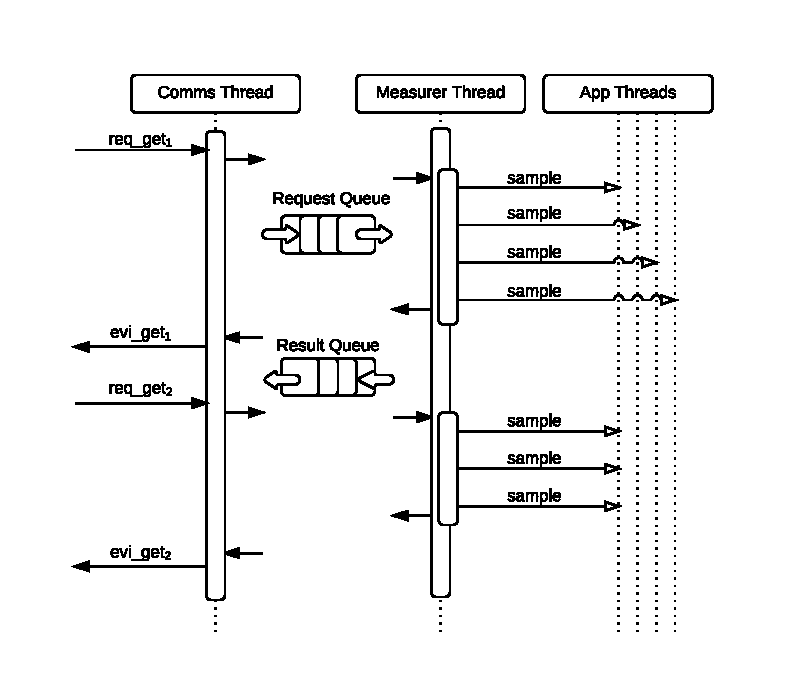
\includegraphics[width=0.9\textwidth]{figures/Measurer_Basic.pdf}
%   \end{center}  
% \end{frame}

% \begin{frame}
%   \frametitle{Measurer - Continuous Sampling}
%   \begin{center}
%   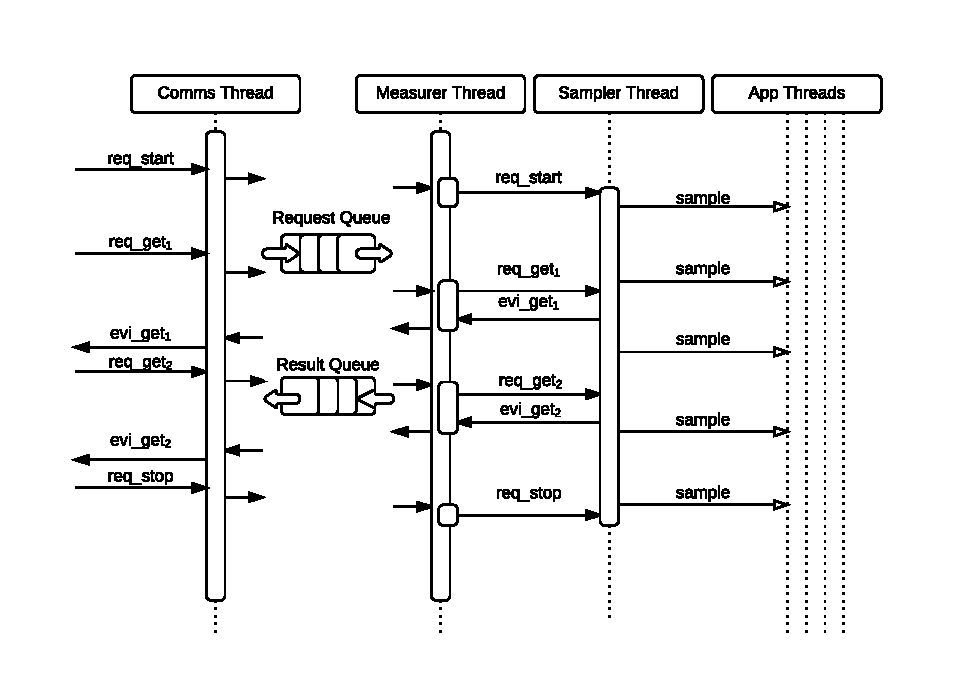
\includegraphics[width=0.9\textwidth]{figures/Measurer_Sampler.pdf}
%   \end{center}  
% \end{frame}

% \begin{frame}
%   \frametitle{Measurer - Continuous Instrumentation}
%   \begin{center}
%   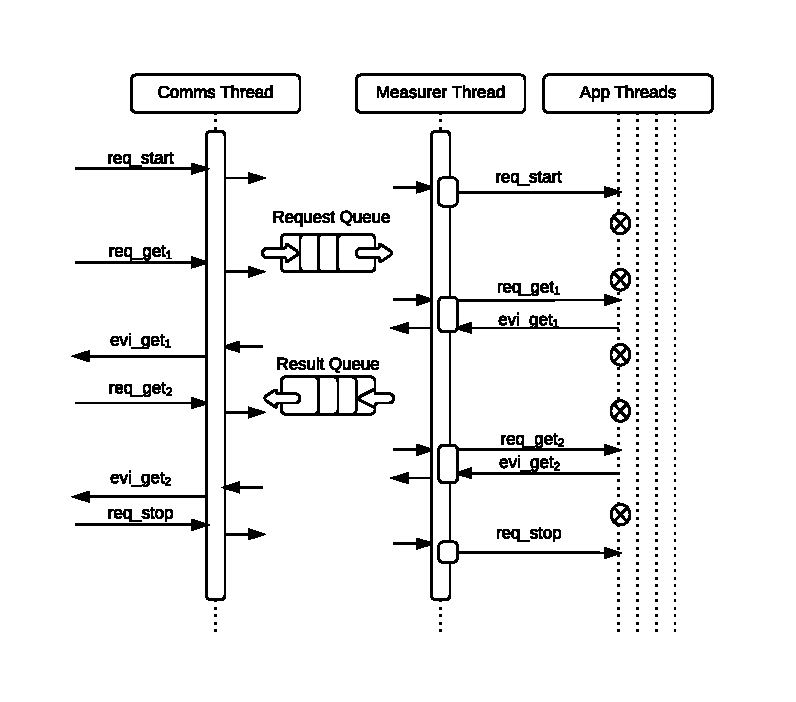
\includegraphics[width=0.9\textwidth]{figures/Measurer_Instrumentor.pdf}
%   \end{center}  
% \end{frame}

% \begin{frame}
%   \frametitle{Measurement Approaches}
%   \begin{itemize}
%   \item Current measurer
%     \begin{itemize}
%     \item individual measurement of user variables
%     \item variables specified externally
%     \item measurer thread monitors the stack or heap contents
%     \end{itemize}
%   \item Use provisioning to fine expected variable values
%     \begin{itemize}
%     \item generate ``golden'' values to define expected state
%     \item track variables at runtie
%     \item dynamic variables are evidence the appraiser uses to ensure
%       application meets expectations
%     \end{itemize}
%   \item Use static analysis to find expected behavior
%     \begin{itemize}
%     \item generate a ``golden'' static callgraph and provide this to the
%       appraiser
%     \item track the dynamic callgraph during execution
%     \item dynamic callgraph is evidence the appraiser uses to ensure
%       application meets expectations
%     \end{itemize}   
%   \end{itemize}
% \end{frame}

% \begin{frame}
%   \frametitle{Communication Mechanisms}
%   \begin{itemize}
%   \item Exploring standard communication mechanisms
%     \begin{itemize}
%     \item Sockets for processes
%     \item \emph{vchan} for IVC within Xen instances
%     \item TCP/IP for IVC between Xen instances
%     \end{itemize}
%   \item Developing standard abstract communication concept
%     \begin{itemize}
%     \item $A->B:M\; on\; c$ is the abstraction users should see
%     \item independent of the type of communication
%     \item manage failure and time-out behind the scenes
%     \item JSON structures for all data communicated
%     \item type preserving communication
%     \end{itemize}
%   \item Armor Authority provides services among  VMs
%     \begin{itemize}
%     \item name services, migration services, certificate authority
%     \item as small as possible
%     \item reuse wherever possible
%     \end{itemize}
%   \end{itemize}
% \end{frame}

% \begin{frame}
%   \frametitle{Example Communication Activity}
%   \framesubtitle{CA communication}

% \begin{itemize}
% \item Attester
%   \begin{itemize}
%   \item creates an $AIKCertRequest$ containing $ID$ and $\public{AIK}$
%   \item converts $AIKCertRequest$ to JSON
%   \item JSON sent as POST request to certificate authority
%   \item $AIKCertRequest$ $->$ JSON $->$ UTF8 $->$ POST body bytes
%   \end{itemize}
% \item Certificate Authority
%   \begin{itemize}
%   \item POST body bytes $\rightarrow$ UTF8 $\rightarrow$ JSON $\rightarrow$ $AIKCertRequest$
%   \item looks up \public{EK} associated with $ID$
%   \item $AIKCert$ is \sign{\public{AIK}}{CA}
%   \item generates session key $K$ and encrypts with \public{EK}
%   \item $AIKCert$ encrypted with $K$
%   \item $CAResponse$ converted to JSON and sent as response
%   \end{itemize}
% \end{itemize}

% \end{frame}

% \begin{frame}{\ca{} communication continued}
% Properties
% \begin{itemize}
% \item {\ca{} only responds to receiving an $AIKCertRequest_{JSON}$ }
% \item {The CACert can \emph{only} be decrypted by knowing $K$ (and therefore \private{EK})}
% \end{itemize}
% $\linebreak$
% Appraiser Knowledge after receiving Cert:
% \begin{itemize}
% \item {signature on $AIK$ ensures it was \ca{} who generated signature
% }
% +
% \item {only an entity knowing \private{EK} could decrypt and send the CACert
% }
% $\linebreak$
% =
% \item {\textbf{Attester is using a registered TPM}}

% \end{itemize}

% \end{frame}

\begin{frame}[fragile]
  \frametitle{Negotiation}

  \begin{block}{Protocol}
  \begin{alltt}
  do \{ send t \$ r;
       q <- receive t;
       e <- case \{p:q | policy?(p)\} of
              \(\emptyset\) : None
              p : send t \$ choose(p)
            end;
       case e of 
         Some v : appraise(v)
         None : None
       end
  \}
\end{alltt}
\end{block}

\begin{block}{Proposals}
  \[
  \{\tuple{E_0,P_0},\tuple{E_1,P_1},\ldots,\tuple{E_n,P_n}\}
  \]
\end{block}

\end{frame}

\begin{frame}[fragile]
  \frametitle{Single Realm Attestation}

\begin{block}{Protocol}
\begin{alltt}
  do \{ id <- getVCID;
       sig <- getSigFileEvidence;
       src <- getSigFileSrc;
       e <- createEvidence(id,sig,src);
       returnEvidence(e)
  \}
\end{alltt}
\end{block}

\begin{block}{Evidence}
\[\evidence{(id,sig,src)}{\hash{(id,sig,src)},PCRComp_0}{AIK_0}\]
\end{block}

\end{frame}

\begin{frame}[fragile]
  \frametitle{Multi-Realm Attestation}

\begin{block}{Protocol}
\begin{alltt}
  do \{ id <- getVCID;
       sig <- getSigFileEvidence;
       src <- getSigFileSrc;
       srcEvidence <- send src \$ r;
       e <- createEvidence(id,sig,src,srcEvidence)
       returnEvidence(e)
  \}
\end{alltt}
\end{block}

\begin{block}{Evidence}
\[b=\evidence{(e)}{\hash{e},PCRComp_1}{AIK_1}\]
\[\evidence{(id,sig,src,b)}{\hash{(id,sig,src,b)},PCRComp_0}{AIK_0}\]
\end{block}

\end{frame}

\begin{frame}
  \frametitle{Current Status}

  \begin{center}
  \emph{\color{kublue}Completed four demonstrations culminating in
    running an attestation protocol in response to an attestation
    request.}
  \end{center}

  \begin{itemize}
  \item Attestation and Appraisal development
    \begin{itemize}
    \item CA-Based attestation protocol execution example
    \item integration with Berlios TPM 1.2 emulator
    \item simple dynamic appraisal of attestation results
    \end{itemize}
  \item Measurement development
    \begin{itemize}
    \item on demand Java program measurement
    \item HotSpot-based Java VM run time measurements
    \item standard mechanism for extending measurement capabilities
    \end{itemize}
  \item Communication infrastructure
    \begin{itemize}
    \item vchan, TCP/IP and socket communication infrastructure
    \item language-based interface with TPM 1.2
    \item JSON-based data exchange formats
    \item initial certificate authority API
    \end{itemize}
  \end{itemize}
\end{frame}

\section{Year 2 Goals and Milestones}

\begin{frame}
  \frametitle{Goals and Milestones for 2015}

  \begin{center}
    {\color{kublue}Increased functionality and robustness}
  \end{center}

  \begin{itemize}
  \item Push to the cloud
    \begin{itemize}
    \item integration with OpenStack
    \item migration across Xen instances
    \item vTPM function migration
    \end{itemize}
  \item Establish roots-of-trust and trust argument
    \begin{itemize}
    \item measured launch and remeasurement of ArmoredSoftware
    \item establish trust in the Xen/OpenStack infrastructure
    \end{itemize}
  \item Executable protocol representation and protocol semantics
    \begin{itemize}
    \item richer protocol collection
    \item evidence of proper execution
    \item protocol-centered appraisal
    \end{itemize}
  \item Operational, integrated vTPM prototype
    \begin{itemize}
    \item integration with TPM 1.2
    \item find and integrate, not build (we hope)
    \end{itemize}
  \end{itemize}
\end{frame}

\begin{frame}
  \frametitle{Goals and Milestones for 2015}

  \begin{itemize}
  \item More robust communication and system services
    \begin{itemize}
    \item Armor Authority prototype
    \item Certificate Authority integration
    \item communications management
    \end{itemize}
  \item More capable measurement
    \begin{itemize}
    \item compiler directed measurement
    \item continuous measurement of trends
    \end{itemize}
  \item More interesting download-able demonstration
    \begin{itemize}
    \item sponsor-defined problem
    \item more realistic attacker model
    \end{itemize}
  \end{itemize}
\end{frame}

% \section{Questions and guidance}

% \begin{frame}
%   \frametitle{Questions and Guidance}

%   \begin{itemize}
%   \item What should we be watching and integrating with?
%     \begin{itemize}
%     \item operational vTPM infrastructure
%     \item infrastructure measured boot
%     \item certificate authorities
%     \end{itemize}
%   \item What demonstration problems are relevant?
%     \begin{itemize}
%     \item federated trust
%     \item trust in the infrastructure
%     \item trust among application collections
%     \end{itemize}
%   \item What would convince you to work a problem with us?
%   \end{itemize}
% \end{frame}

\nocite{Coker::Principles-of-R,Haldar:04:Semantic-Remote,Fabrega:1999aa,Ryan:09:Introduction-to}

\begin{frame}
  \frametitle{References}
  \bibliography{overview}
\end{frame}

\end{document}

